\chapter{Applications}

\par
Les applications possibles à partir des cartes de saillance sont illimitées. Eakta Jain, professeur assistante à l'université de de Floride, a déjà travaillé avec Olivier et a pu nous apporter son expérience grâce aux différents projets d'applications basés sur le mouvement du regard qu'elle a réalisé \cite{eaktalab}. Ses projets liés au regard humain sont souvent appliqués aux comics qui a des similarités avec la peinture.

\section{Recherche d'application}

\par
Afin de déterminer quelle application il serait intéressant de développer, il faut faire une recherche de ce qui existe déjà ou inventer autre chose. Je vais présenter ici les différentes pistes qui ont été envisagées et expliquer notre choix final.

\par
Pour ajouter du mouvement, il existe des logiciels qui permettent de générer des plotagraphes. Basé sur les cinémagraphes, qui sont des mélanges d'images et de vidéos, les plotagraphes permettent d'ajouter du mouvement à partir de l'image seule. En revanche il faut ajuster à la main les zones à mouvoir donc difficilement automatisable et le résultat n'est impressionnant que sur les fluides (eau, nuages, fumée...).

\par
Eakta a un projet de segmentation des différentes parties d'un comic pour animer les personnes qui parle et ajouter du son \cite{segmentationcomics}. La segmentation est obtenue à partir du chemin visuel aquis par occulométrie. Une idée intéressante mais difficlement adaptable à toutes les peintures car trop détaillée.

\par
Un autre projet d'Eakta appelé "Predicting Moves-on-Stills for Comic Art using Viewer Gaze Data" \cite{kenburns} ajoute un effet de Ken Burns sur des pages de comics en fonction des prédictions du mouvement du regard du spectateur. Cet un effet intéressant et facile à mettre en place. C'est la piste vers laquelle on se dirigera et que l'on détaillera dans la partie suivante. Il existe aussi une version 3D de cet effet \cite{kenburns3D} qui est très impressionant mais est compliqué a mettre en place et difficile à mettre en relation avec la carte de saillance.

\newpage
\section{Effet Ken burns}

\par
L'effet Ken Burns est représenté par un mouvement de caméra (panoramique, zoom ou rotation) sur une image fixe. L'ajout de mouvement et d'animation permet de garder l'attention du spectateur. C'est un effet qui est très régulièrement utilisé dans les documentaires, dans les journeaux ou tout simplement dans les diaporamas photos. 

\begin{figure}[ht]
    \centering
    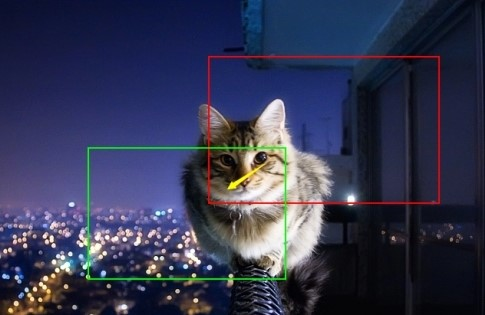
\includegraphics[width=0.7\linewidth]{datas/kenburnseffect.jpg}
    \caption{Exemple d'effet Ken Burns avec panoramique du cadre rouge vers le cadre vert}
    \label{kenburnsexemple}
\end{figure}

\par
J'ai donc décidé de partir sur un effet Ken Burns comme projet d'application. Mon but ici est que le mouvement de la caméra suive celui d'un \oe{}il humain. On est capable de généré un chemin visuel à partir d'une carte de saillance grâce à un modèle saccadique. J'ai pu en utiliser un créé par Olivier Le Meur \cite{saccadicmodel} disponible sur le gitlab de l'équipe Percept. Ainsi à partir d'une peinture on obtient une carte de saillance grâce au modèle de saillance, puis le chemin visuel grâce au modèle saccadique et enfin un effet Ken Burns qui suit le chemin visuel.

\par
Je me suis donc lancé dans la réalisation d'un programme en Python qui en entrée prend une peinture et le chemin visuel associé pour en sortie obtenir une vidéo avec l'effet Ken Burns. Le principe de base est d'avoir une caméra qui se déplace dans l'image et qui enregistre ses déplacements à la fréquence de la vidéo de sortie.

\par
Pour les mouvements j'ai codé le zoom et le panoramique, la rotation ici n'a pas forcément d'intérêt. J'ai d'abord commencé par créer l'effet de zoom qui consiste à redimensionner l'image tout en gardant la résolution de la caméra identique. Donc par exemple pour un zoom x2 je double la taille de l'image mais je garde celui de la caméra sur les dimensions d'origine. Une fois zoomé, le but est de se déplacer de fixation en fixation en suivant le chemin visuel. Afin d'obtenir des mouvements lisses et de pouvoir gérer les bords proprement je précalcule la position finale de ma caméra puis je fais bouger la caméra de mon point d'origine vers la position finale. En fusionnant les deux mouvements on peut créer un zoom sur un point précis de l'image.

\par
Dans un premier temps le mouvement était trop linéaire ce qui a pour effet de donner un rendu final assez pauvre et saccadé. Pour lisser les mouvements j'ai appliqué un effet de ease-in-out. Cela permet d'avoir une accélération progressive au début du mouvement et une décélération progressive à la fin. Au lieu d'avoir une interpolation linéaire (graphe \ref{subfig:lineaire}), c'est-à-dire que la caméra se déplace de la même distance entre chaque image d'un plan à un autre, ici on a une interpolation avec de petites distances en début et en fin de parcours mais de grandes distances en milieu de parcours (graphe \ref{subfig:ease}).

\begin{figure}[ht]
    \centering
    \begin{subfigure}{.49\textwidth}
        \centering
        \begin{tikzpicture}
            \begin{axis}[every axis plot post/.append style={
              mark=none,domain=0:60,samples=50,smooth},
                % All plots: from -2:2, 50 samples, smooth, no marks
              axis x line*=bottom, % no box around the plot, only x and y axis
              axis y line*=left, % the * suppresses the arrow tips
              enlargelimits=upper] % extend the axes a bit to the right and top
              \addplot {x/60};
            \end{axis}
            \end{tikzpicture}
        \caption{Linéaire}
        \label{subfig:lineaire}
    \end{subfigure}
    \begin{subfigure}{.49\textwidth}
        \centering
        \begin{tikzpicture}
            \begin{axis}[every axis plot post/.append style={
              mark=none,domain=0:60,samples=50,smooth},
                % All plots: from -2:2, 50 samples, smooth, no marks
              axis x line*=bottom, % no box around the plot, only x and y axis
              axis y line*=left, % the * suppresses the arrow tips
              enlargelimits=upper] % extend the axes a bit to the right and top
              \addplot {-(cos(pi*x)-1)/2};
            \end{axis}
            \end{tikzpicture}
        \caption{Ease-in-out}
        \label{subfig:ease}
    \end{subfigure}
    \caption{Graphes représentant les coefficients d'interpolations pour 60 images}
    \label{fig:graphes}
\end{figure}

\comment{Faire montage vidéo pour montrer différence avec lien en annexe ?}

\par
Pour améliorer l'application un concept d'intelligence artificielle qui décrit ce qu'elle voit a été pensé. L'idée ici serait d'ajouter aux vidéos des sous-titres automatiques générés par du machine learning qui décrivent ce qui est représenté. Il en existe qui fonctionne pour des scènes naturelles avec par exemple le modèle Neuraltalk2 de Karpathy (\linkrename{démo}{http://cs.stanford.edu/people/karpathy/neuraltalk2/demo.html}). Malheureusement la description des éléments dans les peintures est assez désastreuse. De plus si on veut entrainer le modèle avec des mots relatif à la peinture, il nous faut une base de données de mots associés à des éléments abstraits ce qui est très compliqué a mettre en place.